\scanpage{87}
% archive foliation: 86; landscape manuscript on music paper
$E=$ module d'\unsure{une|un} ``rep. \unsure{vraie|naïve}''
\[
\begin{array}{ll}
\text{de}&\deleted{M}\ M\\
\text{de}&\mathfrak g\\
\text{de}&\mathfrak g'\\
\text{de}&G\\
\text{de}&G'
\end{array}
\qquad
\begin{array}{l}
\mathfrak g=\underline{\operatorname{Lie}}G\\
\mathfrak g'=\operatorname{Lie}G'
\end{array}
\]

1.2. Données équivalentes

a) fibré \deleted{\unsure{proj. $P$}} \inserted{en droites}
proj. $P$ sur $X$, avec section marquée $\sigma$

b) Structure d'extension
\[
0\longrightarrow\Omega\longrightarrow\mathcal L
\longrightarrow\underline O_X\longrightarrow0
\]
$\Omega$ inversible

c) Algèbre d'Azumaya de rg 4 $M$, avec idéal
\inserted{$\unsure{\mathfrak a}$} ``spécial''
$\unsure{\mathfrak a_\sigma|\mathfrak a}$

d) $\mathfrak g$ avec ss.-Alg. de Borel $\mathcal L$

\[
\begin{array}{llll}
\text{d')}&\mathfrak g'&\rule{4cm}{.3pt}&\mathcal L'\\
\text{e)}&G&\rule{1.8cm}{.3pt}\ \text{gr.}\ \rule{1.5cm}{.3pt}&B\\
\text{e')}&G'&\rule{1.8cm}{.3pt}\ \text{gr.}\ \rule{1.5cm}{.3pt}&B'
\end{array}
\]
\deleted{f) Une \unsure{$O_X$ Algèbre|Ext($O_X$)} avec une
\unsure{$P_2$|$\Omega_2$} \unsure{marquée}
\unsure{rigidité|rigidifiée} \unsure{d'extension 2|d'ordre 2},
de ``rang'' 1}
\inserted{\unsure{trivialisée|tr. qui est $e'$}}

\inserted{à a)} est associé $\unsure{L:=\underline L|\underline L}$
faisc. inv. de degré rel. $(1)$,
\uline{rigidifié} par $\sigma^*(L)\simeq\underline O_X$. Alors
\[
\begin{aligned}
+\quad\mathcal L&=f_*(L),\quad\text{avec structure d'ext. évidente}\\
&\simeq f_*\bigl(L/\unsure{\mathcal I^2L|\mathcal IL}\bigr)\\
&\simeq\sigma^*(P^1(L))
\end{aligned}
\]
($\mathcal I=$ Idéal de $\sigma(X)$ dans $P$)

$P=\mathbb P(\mathcal L)$ avec section corresp. au quotient
$\underline O_X$ de $\mathcal L$

$=$ clôture projective du torseur sous $W(\Omega)$ défini par l'extension.

et $M=\operatorname{End}\mathcal L$, avec idéal annulateur de $\Omega$
\margin{\deleted{(\unsure{formes splittées|formes déployées})}}
\[
\mathfrak g=M/\underline O_X\simeq\operatorname{Sym}^2(\mathcal L)
\otimes\Omega^{-1}\qquad(\mathrm{NB}\ \det\mathcal L\simeq\Omega)
\]
Or $\operatorname{Sym}^2\mathcal L$ est filtré par
\inserted{(décro)} $\underline O_X,\Omega,\Omega^2$,
donc $\operatorname{Sym}^2\mathcal L\otimes\Omega^{-1}$ filtré par (croiss)
\[
\begin{array}{ccc}
\Omega&\underline O_X&\Omega^{-1}\\
\Vert&\Vert&\Vert\\
\operatorname{Fil}_1&\operatorname{Fil}_2/\operatorname{Fil}_1
&\operatorname{Fil}_3/\operatorname{Fil}_2=\\
\Vert&\Vert&\Vert\\
\operatorname{gr}_1&\operatorname{gr}_2&\operatorname{gr}_3
\end{array}
\]
\figure{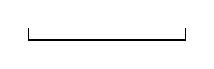
\begin{tikzpicture}\draw (0,.15)--(0,0)--(2,0)--(2,.15);\end{tikzpicture}}
\margin{\unsure{exprimer|expliquer} aussi \unsure{ce|de}
$(\mathfrak g,\mathcal L)$ \unsure{à partir|par}
\[
0\longrightarrow\Omega\longrightarrow\mathcal L
\longrightarrow\underline O_X\longrightarrow0
\]
$(\Omega=\mathcal L_{\unsure{\mathrm{un}}},\ldots)$}

% right-hand column, continuing the filtration computation
où
\[
\begin{aligned}
\operatorname{Fil}_2
&=\Omega^{-1}\otimes
\underbrace{(\operatorname{Ker}\operatorname{Sym}^2\mathcal L
\longrightarrow\operatorname{Sym}^2 O)}_{\simeq\Omega\otimes\mathcal L}\\
&\simeq\mathcal L
\end{aligned}
\]
donc on a
\[
\underset{\Omega}{\underbrace{\Omega}}\subset
\underset{\underline O_X}{\underbrace{\mathcal L}}\subset
\underset{\Omega^{-1}}{\underbrace{\mathfrak g}}
\]
et $\mathcal L$ est une ss.-Alg. de Borel
($\Omega$ \unsure{sa part.|rad.} unipotente)

\margin{\uline{NB} Pour forme de Killing,
$\Omega$ et $\mathcal L$ orth. l'un à l'autre, \inserted{2 inv.!}}

On n'explicite pas $(\mathfrak g',\mathcal L')$
($\simeq(\mathfrak g,\mathcal L)$ si 2 inv.), pour $(G,B)/(G',B')$ on a
\[
G'=\underline{SL}_{\Omega}\mathcal L,\qquad
B'\inserted{\subset G'}=\text{Stabilisateur de }\Omega
\]
$G,B$ déduits par passage au quot. par Centre $\mu_2$

\margin{\uline{NB}
\[
\mathfrak g/\Omega\simeq\unsure{\mathcal L^\vee|\mathcal L}
\]
\[
\mathcal L^\vee\simeq\mathcal L\otimes\det\mathcal L^{-1}
\simeq\mathcal L\otimes\Omega^{-1}
\]
avec filtration opposée

vérifier!}
\figure{\begin{tikzpicture}[x=1cm,y=1cm]
\draw (0,0) to[bend right=40] (-.5,2)
to[bend right=40] (2.3,2.6) to[bend right=40] (2.6,.5)
to[bend right=20] (0,0);
\draw[->] (2,3) to[bend left=25] (2.5,2);
\draw (2.3,2.6)--(4,2.6);
\end{tikzpicture}}

[\uline{1.\deleted{3}\inserted{4}.} Supposons $X/S$, et considérons des
\uline{connexions} \inserted{rel. $S$} sur les objets du type envisagé
dans 1.1, \unsure{mais augmentés|munis également}
\unsure{par} \inserted{la donnée d'}une structure 1.2.
Ainsi, on \unsure{consid.|considère} des couples
\[
(P,\sigma,C)
\]
\[
\left\{\begin{array}{l}
P\text{ fibré en droites projectives sur }X\\
\sigma\text{ section}\\
C\text{ connexion de }P\text{ rel. à }S.
\end{array}\right.
\]
(mais on ne suppose pas $\sigma$ plat.)
\margin{\uline{faux}}

\unsure{Il nous sera peut-être commode d'expliciter|Il me sera peut-être commode d'expliciter}
en termes de $(\mathcal L,\Omega)$ i.e.
\[
0\longrightarrow\Omega\longrightarrow\mathcal L
\longrightarrow\underline O_X\longrightarrow0
\]
(qui donne $(P,\sigma)$, \inserted{d'où $(\mathfrak g,\mathcal L)$, comme expliqué}
et d'une connexion de $\mathfrak g$.
\deleted{\unsure{On note qu'on}}
]

